\documentclass[tikz,border=12pt]{standalone}
\usepackage[T1]{fontenc}
\usepackage{mathptmx}
\usepackage{tikz}
\usetikzlibrary{arrows.meta,positioning,shapes.geometric,calc}

\definecolor{boxfill}{HTML}{EEECFE}
\definecolor{boxdraw}{HTML}{5B4B8A}
\definecolor{pillfill}{HTML}{F6F5FD}
\definecolor{pilldraw}{HTML}{7A6EB0}

\begin{document}
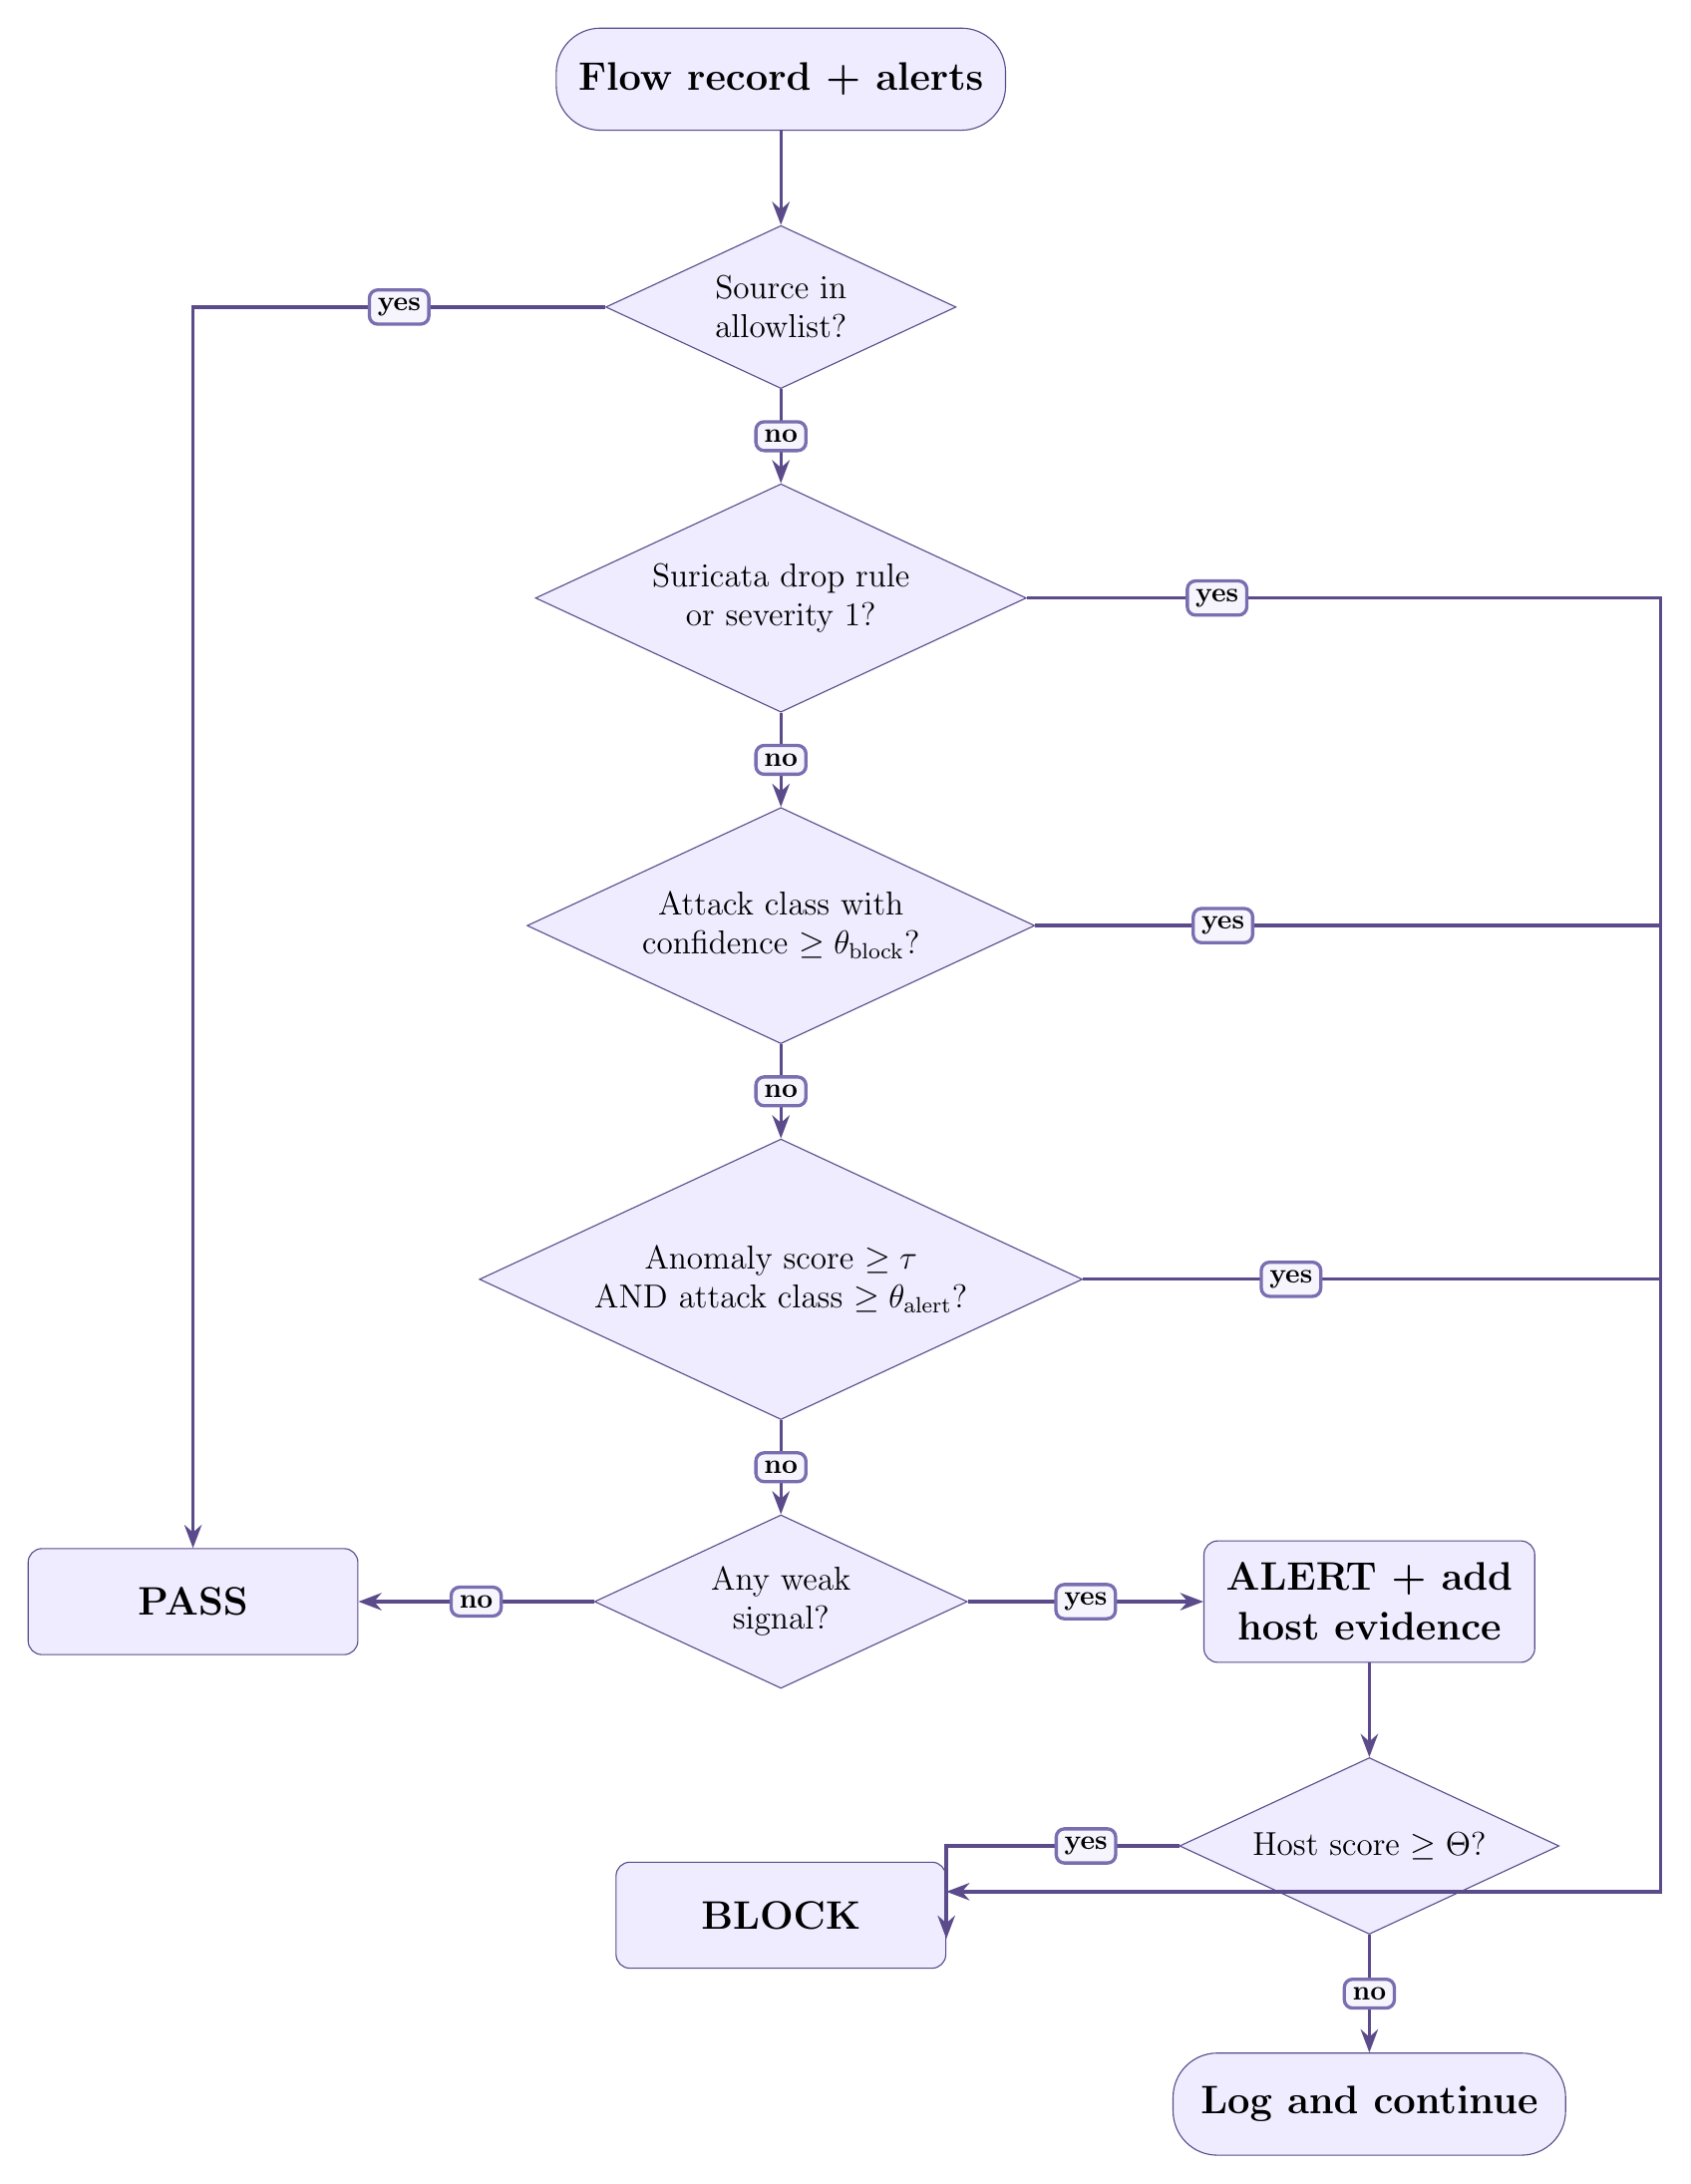
\begin{tikzpicture}[
  font=\large,
  >=Stealth,
  node distance=12mm and 26mm,
  startnode/.style={draw=boxdraw, fill=boxfill, rounded corners=16pt,
    align=center, inner sep=8pt, minimum width=5.0cm, minimum height=1.3cm, font=\Large\bfseries},
  decision/.style={diamond, draw=boxdraw, fill=boxfill, aspect=2.15,
    align=center, inner sep=5pt, font=\large},
  action/.style={draw=boxdraw, fill=boxfill, rounded corners=5pt,
    align=center, inner sep=8pt, minimum height=1.35cm, minimum width=4.2cm, font=\Large\bfseries},
  tag/.style={fill=pillfill, draw=pilldraw, rounded corners=3pt, inner sep=3pt, font=\normalsize\bfseries},
  arr/.style={->, very thick, draw=boxdraw}
]

% Central vertical column
\node[startnode] (in) {Flow record + alerts};
\node[decision, below=12mm of in] (allow) {Source in\\allowlist?};
\node[decision, below=12mm of allow] (l1) {Suricata drop rule\\or severity 1?};
\node[decision, below=12mm of l1] (l3) {Attack class with\\confidence $\ge \theta_{\mathrm{block}}$?};
\node[decision, below=12mm of l3] (l2l3) {Anomaly score $\ge \tau$\\AND attack class $\ge \theta_{\mathrm{alert}}$?};
\node[decision, below=12mm of l2l3] (weak) {Any weak\\signal?};

% Bottom Action nodes
\node[action, left=30mm of weak] (pass) {PASS};
\node[action, below=22mm of weak] (block) {BLOCK};

% Right branch: Alert + Host score
\node[action, right=30mm of weak] (alert) {ALERT + add\\host evidence};
\node[decision, below=12mm of alert] (host) {Host score $\ge \Theta$?};
\node[startnode, below=15mm of host] (log) {Log and continue};

% Central column connectors
\draw[arr] (in) -- (allow);
\draw[arr] (allow) -- node[tag, midway] {no} (l1);
\draw[arr] (l1) -- node[tag, midway] {no} (l3);
\draw[arr] (l3) -- node[tag, midway] {no} (l2l3);
\draw[arr] (l2l3) -- node[tag, midway] {no} (weak);

% Left branch to PASS (no crossings)
\draw[arr] (allow.west) -| node[tag, pos=0.25] {yes} (pass.north);
\draw[arr] (weak.west) -- node[tag, midway] {no} (pass.east);

% Weak signal branch
\draw[arr] (weak.east) -- node[tag, midway] {yes} (alert.west);

% Right branch: YES to BLOCK from detection layers
% Routed cleanly around alert to keep the diagram fully planar
\coordinate (bus) at ([xshift=16mm]alert.east);
\draw[very thick, draw=boxdraw] (l1.east) -| node[tag, pos=0.15] {yes} (bus);
\draw[very thick, draw=boxdraw] (l3.east) -| node[tag, pos=0.15] {yes} (bus);
\draw[very thick, draw=boxdraw] (l2l3.east) -| node[tag, pos=0.18] {yes} (bus);
\draw[arr] (bus) |- ([yshift=3mm]block.east);

% Host score branch
\draw[arr] (alert) -- (host);
\draw[arr] (host.west) -| node[tag, pos=0.2] {yes} ([yshift=-3mm]block.east);
\draw[arr] (host.south) -- node[tag, midway] {no} (log.north);

\end{tikzpicture}
\end{document}
